\documentclass[11pt]{amsart}

\usepackage[usenames,dvipsnames,svgnames,table]{xcolor}
\usepackage[colorlinks=true, pdfstartview=FitV, linkcolor=blue, citecolor=blue, urlcolor=darkblue]{hyperref}

%\usepackage{addfont}
%\addfont{OT1}{rsfs10}{\rsfs}

\usepackage{geometry}                % See geometry.pdf to learn the layout options. There are lots.
\geometry{letterpaper}                   % ... or a4paper or a5paper or ...
%\geometry{landscape}                % Activate for for rotated page geometry
%\usepackage[parfill]{parskip}    % Activate to begin paragraphs with an empty line rather than an indent
\usepackage{graphicx}
\usepackage{mathrsfs}
\usepackage{amssymb}
\usepackage{amsfonts}
\usepackage{mathrsfs}
\usepackage{epstopdf}
\usepackage{lscape}
\usepackage[utf8]{inputenc}
\usepackage{tikz,caption}
\DeclareGraphicsRule{.tif}{png}{.png}{`convert #1 `dirname #1`/`basename #1 .tif`.png}
\usepackage{enumitem}
\setlist[itemize]{leftmargin=2em}
\setlist[enumerate]{leftmargin=2em}
\usepackage{booktabs}
\usepackage{multirow}
\usepackage{mathtools}
\usepackage[linesnumbered,ruled]{algorithm2e}

\definecolor{darkblue}{rgb}{0.0,0,0.7} % darkblue color
\definecolor{darkred}{rgb}{0.7,0,0} % darkred color
\definecolor{darkgreen}{rgb}{0, .6, 0} % darkgreen color

% Dark red emphasis
\newcommand{\defncolor}{\color{darkred}}
\newcommand{\defn}[1]{{\defncolor\emph{#1}}} % emphasis of a definition

\newtheorem{theorem}{Theorem}[section]
\newtheorem{prop}[theorem]{Proposition}
\newtheorem{cor}[theorem]{Corollary}
\newtheorem{lemma}[theorem]{Lemma}
\newtheorem{conj}[theorem]{Conjecture}
\theoremstyle{definition}
\newtheorem{definition}[theorem]{Definition}
\newtheorem{example}[theorem]{Example}
\newtheorem{remark}[theorem]{Remark}
\numberwithin{equation}{section}

\usepackage[colorinlistoftodos]{todonotes}
\newcommand{\idiot}[1]{\vspace{5 mm}\par \noindent
\marginpar{\textsc{Note}}
\framebox{\begin{minipage}[c]{0.95 \textwidth}
#1 \end{minipage}}\vspace{5 mm}\par}
\newcommand{\mike}[1]{\todo[size=\tiny,color=lime!30]{#1 \\ \hfill --- Mike}}
\newcommand{\nantel}[1]{\todo[size=\tiny,color=red!30]{#1 \\ \hfill --- Nantel}}
\newcommand{\yohana}[1]{\todo[size=\tiny,color=Cyan]{#1 \\ \hfill --- Yohana}}
\newcommand{\farad}[2][]{\todo[size=\tiny,color=ForestGreen!30,#1]{#2 \\ \hfill --- Farad}}
\newcommand{\kelvin}[1]{\todo[size=\tiny,color=RoyalBlue!30]{#1 \\ \hfill --- Kel}}

%remove the comment from the following line to remove all the
% extra proofs:
%\renewcommand{\idiot}[1]{}

\title{Quasi-symmetric harmonics of the exterior algebra}
\author{Nantel Bergeron,
Kelvin Chan,
Yohana Solomon,
Farhad Soltani,
Mike Zabrocki}
\date{Draft November 2021}

\begin{document}

\maketitle

%%%%%%%%%%%%%%%%%%%%%%%%%%%%%%%%%%%%%%
%%%%%%%%%%%%%%%%%%%%%%%%%%%%%%%%%%%%%%
%%%%%%%%%%%%%%%%%%%%%%%%%%%%%%%%%%%%%%
\section{Introduction}


%%%%%%%%%%%%%%%%%%%%%%%%%%%%%%%%%%%%%%
%%%%%%%%%%%%%%%%%%%%%%%%%%%%%%%%%%%%%%
%%%%%%%%%%%%%%%%%%%%%%%%%%%%%%%%%%%%%%
\section{Quasisymmetric invariants on the exterior algebra}

Fix $n$ a positive integer and
let $R_n = {\mathbb Q}[\theta_1, \theta_2, \ldots, \theta_n]$ be the
polynomial ring in anticommuting variables.
The ring $R_n$ is isomorphic to the exterior algebra of a vector
space of dimension $n$.  The variables of this ring satisfy the relations
\[
\theta_i \theta_j = - \theta_j \theta_i \hbox{ if } 1 \leq i \neq j \leq n
\qquad\hbox{and}\qquad \theta_i^2 = 0 \hbox{ for }1 \leq i \leq n~.
\]
Since these conditions impose that a monomial in $R_n$ has no repeated variables,
the monomials are in bijection with subsets of $\{1,2,\ldots, n\}$
and the dimension of $R_n$ is therefore equal to $2^n$.

Denote $[n] := \{1,2, \ldots,n\}$ and
let $A = \{a_1 < a_2 < \cdots < a_r \} \subseteq [n]$.
We define $\theta_A := \theta_{a_1} \theta_{a_2} \cdots \theta_{a_r}$,
then the set $\{ \theta_A \}_{A \subseteq [n]}$ is a basis of $R_n$.

We define an action on monomials of $R_n$ and extend this action linearly.
For each integer $1 \leq i < n$, let $\pi_i$ be an operator on $R_n$
that is defined by
\begin{equation}\label{eq:pi}
\pi_i(\theta_A) = \begin{cases}
\theta_{A} & \hbox{ if } i, i+1 \in A\hbox{ or }i, i+1 \notin A\\
\theta_{A \cup \{i+1\} \backslash \{i\}} & \hbox{ if } i\in A\hbox{ and }i+1 \notin A\\
\theta_{A \cup \{i\} \backslash \{i+1\}} & \hbox{ if } i+1\in A\hbox{ and }i \notin A
\end{cases}~.
\end{equation}
These operators instead of exchanging an $i$ for an $i+1$ like the symmetric group
action, have the effect of shifting the indices of the variables (if possible).  They
are therefore known as quasisymmetric operators.  They were studied in depth by
Hivert \cite{H}.  The operators are not multiplicative on $R_n$ in general since, for example,
\[
\pi_1( \theta_{1} \theta_{2})
= \theta_1 \theta_2
= - \pi_1( \theta_{1}) \pi_1(\theta_{2})~.
\]
They are also not multiplicative when they act on the polynomial ring
in commuting variables.

A polynomial that is invariant under the action of quasisymmetric operators
is said to be quasisymmetric invariant (or just `quasisymmetric').
The quasisymmetric invariants of $R_n$ are
linearly spanned by the elements:
\begin{equation}\label{eq:defF}
F_{1^r}(\theta_1, \theta_2, \ldots, \theta_n) := \sum_{\substack{A \subseteq [n]\\|A|=r}} \theta_A~.
\end{equation}
The symbols $F_{1^r}$ for the elements borrows the notation from the
polynomial ring in commuting variable invariants known as the `fundamental
quasisymmetric polynomials'.  The commuting polynomial quasisymmetric
invariants are indexed by compositions.


\begin{remark}
As expressing polynomials with listing the variables
(e.g. $p(\theta_1, \theta_2, \ldots, \theta_n)$) can be notational cumbersome,
there will be points where we will drop the variables in the expressions
and this will indicate that the polynomials are in the
variables $\theta_1, \theta_2, \ldots, \theta_n$.  There will also
be expressions where some polynomials have fewer variables and there
we will indicate this by listing the variables.
\end{remark}

%%%%%%%%%%%%%%%%%%%%%%%%%%%%%%%%%%%%%%
\subsection{Quasisymmetric functions generate a commutative subalgebra}
In \cite{FLP}, the authors showed that the quasisymmetric functions in
one set of commuting variables and one set of anti-commuting variables
forms a graded Hopf algebra.  This implies that the quasisymmetric functions
in one set of anti-commuting variables are closed under multiplication
and there is one element in this algebra at each non-negative degree.
It follows that for $r, s \geq0$ that there exists a (possibly $0$)
coefficient $a_{r,s}$ such that
\begin{equation}\label{eq:qsalg}
F_{1^r} F_{1^s} = a_{r,s} F_{1^{r+s}}\,.
\end{equation}

\begin{remark}
In  the notation of \cite{FLP}, $F_{1^r}=M_{\dot{0}^r}=L_{\dot{0}^r}$ where $\dot{0}^r=(\dot{0},\dot{0},\ldots,\dot{0})$ a composition of length $r$.
The fermionic degree of $F_{1^r}$ is exactly $r$.
 In~\cite{FLP}, they show that $a_{r,s}$ exists and express it as a sum of $\pm 1$, but they do not give an explicit formula.
Furthermore, they indicate  that $a_{r,s}=(-1)^{rs}a_{s,r}$. Here we shall compute exactly $a_{r,s}$
and the formula shows the subalgebra generated by the $F_{1^r}$ is commutative.
\end{remark}

\begin{prop}\label{prop:comm}
The constants $a_{r,s}$ in Equation~\eqref{eq:qsalg} satisfy the following equation.
$$ a_{r,s}=
\begin{cases}
	0  &\text{if $r,s$ are both odd,}\\
	\\
	\left({\lfloor \frac{r+s}{2} \rfloor \atop \lfloor \frac{r}{2} \rfloor}\right)&\text{otherwise.}
\end{cases}
$$

\begin{proof}
For completeness, we give a proof not assuming any results of~\cite{FLP}. Using Equation~\eqref{eq:defF} we have
$$F_{1^r}F_{1^s}= \sum_{\substack{A \subseteq [n]\\|A|=r}}  \sum_{\substack{B \subseteq [n]\\|B|=s}} \theta_A \theta_B
= \sum_{\substack{C \subseteq [n]\\|C|=r+s}} \Big(\sum_{\substack{A\subseteq C \\|A|=r}} (-1)^{|\{b<a\,|\,a\in A,\, b\in C\setminus A\}|} \Big) \theta_C\,.
$$
To see the second equality, we remark that the product $\theta_A\theta_B=0$ if $A\cap B\ne \emptyset$. Furthermore if $A\cap B= \emptyset$, then for $C=A\cup B$
we have $B=C\setminus A$ and  $\theta_A\theta_B=(-1)^{|\{b<a\,|\,a\in A, b\in C\setminus A\}|} \theta_C$, where the sign is the number of interchanges needed to sort $A$ followed by $B$ into $C$.
This does not depend on the value of the element of $C$, but only on how $A$ is chosen inside $C$. This shows that we get the same coefficient for all $C$ of size $r+s$ and therefore $F_{1^r} F_{1^s} = a_{r,s} F_{1^{r+s}}$ with
\begin{equation}\label{eq:signa}
a_{r,s}=\sum_{\substack{A\subseteq \{1,2,\ldots, r+s\}\\ |A|=r}}
(-1)^{|\{1\le b<a\le r+s\,|\,a\in A, b\not\in A\}|}
\end{equation}
by choosing $C=\{1,2,\ldots,r+s\}$. Let ${C\choose r}=\{A\subseteq C, |A|=r\}$. We define a sign-reversing involution $\Phi\colon {C\choose r}\to{C\choose r}$ as follow.
For $A\in  {C\choose r}$, let $\gamma(A)=\gamma_1\gamma_2\cdots\gamma_{r+s}\in\{0,1\}^{r+s}$, be the sequence such that
 $\gamma_i=1$ if $i\in A$, and $\gamma_i=0$ otherwise.
 We look at the  entries of  $\gamma(A)$ two by two and find the smallest $j$ (if it exists) such that the  pair
 $\gamma_{2j-1}\gamma_{2j}$ is not $00$ or $11$. If there is no such pair, we let $\Phi(A)=A$. If we find such pair we define the involution $\Phi(A)=A'$ where $A'$ is such that $\gamma(A')$ is obtained from $\gamma(A)$ by interchanging $01\leftrightarrow 10$ in position $2j-1,2j$. In the case when  $A'=\Phi(A)\ne A$,
 we let
 $$Inv(A)=\{1\le b<a\le r+s\,|\,a\in A, b\not\in A\}=\{1\le \ell<t\le r+s\,|\,\gamma_\ell=0,\gamma_t=1 \}\,$$
 where $\gamma(A)=\gamma_1\gamma_2\cdots\gamma_{r+s}$.
As long as $(t,\ell)\ne(2j-1,2j)$ there is a bijection between $(t,\ell)\in Inv(A)$ and $(t',\ell)\in Inv(A')$ interchanging the 1 and 0 in posisions $2j-1$ and $2j$.
The pair $(2j-1,2j)$ is in only one of $Inv(A)$ or $Inv(A')$ but not the other. Therefore
$$(-1)^{|\{1\le b<a\le r+s\,|\,a\in A, b\not\in A\}|} = -(-1)^{|\{1\le b<a\le r+s\,|\,a\in A', b\not\in A'\}|}\,.$$
If $\Phi(A)=A$, we have that $|Inv(A)|$ is even since we can match the pairs two-by-two.
Therefore $\Phi$ is a sign reversing involution and all fixed points contribute in Equation~\eqref{eq:signa} with a $+1$. Therefore
$$a_{r,s}=\Big|\big\{ A\in {C\choose r}\big| \Phi(A)=A\big\}\Big|=\left({\lfloor \frac{r+s}{2} \rfloor \atop \lfloor \frac{r}{2} \rfloor}\right)\,,$$
since there is a total of $\lfloor \frac{r+s}{2} \rfloor$ pairs $2j-1,2j$
in a sequence of length $r+s$ and we must have $\lfloor \frac{r}{2} \rfloor$ of them equal to $11$
and all others equal to $00$ in order to get $\Phi(A)=A$.
\mike{add a mention of what that leftover guy is equal to if $r$ is even/odd}
\end{proof}
\end{prop}

The generating series for the coefficients $F(x,y) = \sum_{r,s \ge 0} a_{r,s} x^{r}y^{s}$ is
equal to $\frac{1 + x + y}{1 - x^{2} - y^{2}}$
and the OEIS \cite{OEIS} sequence number is \href{https://oeis.org/A051159}{A051159}.
This can be derived from Proposition \ref{prop:comm} using standard techniques of generating functions.
\mike{TODO: add comment to OEIS sequence}

One consequence of Proposition~\ref{prop:comm} is that $a_{r,s}=a_{s,r}$ for all $r,s\ge 0$. Remark that this does not contradict the fermionic law stating that $a_{r,s}=(-1)^{rs}a_{s,r}$ since $a_{r,s}=0$ when both $r,s$ are odd. Therefore we have shown the following corollary.

\begin{cor}
The subalgebra generated by quasisymmetric invariants $\{F_{1^r}|r\ge 0\}$ is commutative.\hfill$\square$
\end{cor}

%%%%%%%%%%%%%%%%%%%%%%%%%%%%%%%%%%%%%%
\subsection{The ideal generated by the quasisymmetric invariants}

Define an ideal of $R_n$ generated by the quasisymmetric invariants as
\[
I_n := \left< F_{1^r}(\theta_1, \theta_2, \ldots, \theta_n) : 1 \leq r \leq n \right>
\]

\begin{remark}
Note that since the operators $\pi_i$ are not multiplicative, it
is unlikely to be the case that $I_n$ as an ideal is invariant
under the action of the $\pi_i$.  Indeed, we find that for $n=4$,
\[
\theta_2 F_{1}(\theta_1, \theta_2, \theta_3, \theta_4) =
-\theta_1 \theta_2 + \theta_2 \theta_3 + \theta_2 \theta_4
\]
and if we apply $\pi_1$ to this element, we obtain
\[
\pi_1(\theta_2 F_{1}(\theta_1, \theta_2, \theta_3, \theta_4)) =
-\theta_1 \theta_2 + \theta_1 \theta_3 + \theta_1 \theta_4
\]
and this can be shown to not be in $I_4$.
\end{remark}

The \emph{exterior quasisymmetric coinvariants} are defined to be
\nantel{and is it really coinvariant? (since the ideal is not invariant)}
\mike{no, but the generators are quasi-invariant.  Does it merit
a footnote as we did for EQH?}
\[
EQC_n := R_n/I_n~.
\]


%%%%%%%%%%%%%%%%%%%%%%%%%%%%%%%%%%%%%%
\subsection{Differential operators on the exerior algebra}\label{ssec:harm}
We can define a set of differential operators on $R_n$ which
will permit us to define the orthogonal complement to the
ideal and a notion of quasisymmetric harmonics.

The operators $\partial_{\theta_i}$ act on monomials in $R_n$
by
\[
\partial_{\theta_i}( \theta_A ) = \begin{cases}
(-1)^{\#\{ j \in A: j<i\}}\theta_{A \backslash \{i\}}&\hbox{ if }i \in A\\
0&\hbox{ if }i \in A
\end{cases}~.
\]

The operators can equally be characterized by their commutation
relations
\[
\partial_{\theta_i} \partial_{\theta_j}=-\partial_{\theta_j} \partial_{\theta_i}
\hbox{ if } 1 \leq i \neq j \leq n
\qquad\hbox{and}\qquad
\partial_{\theta_i}^2 = 0\hbox{ for }1 \leq i \leq n
\]
\[
\partial_{\theta_i} \theta_j=-\theta_j \partial_{\theta_i}
\hbox{ if } 1 \leq i \neq j \leq n
\qquad\hbox{and}\qquad
\partial_{\theta_i} \theta_i = 1\hbox{ for }1 \leq i \leq n~.
\]

For a monomial $\theta_A = \theta_{a_1} \theta_{a_2} \cdots \theta_{a_r}$,
let $\overline{\theta_A} = \theta_{a_r} \theta_{a_{r-1}} \cdots \theta_{a_1}$ represent
reversing the order of the variables in the monomial.  Extend this notation to both
differential operators and polynomials (and polynomials of differential operators)
by extending the notation linearly.

We can define an inner product on $R_n$ by setting for $p,q \in R_n$.
\[
\left< p, q \right> = \overline{p(\partial_{\theta_1}, \partial_{\theta_2}, \ldots, \partial_{\theta_n})}
q( \theta_1, \theta_2, \ldots, \theta_n)|_{\theta_1=\theta_2 = \ldots=\theta_n=0}~.
\]
The monomials of $R_n$ form an orthonormal basis of the space with respect to this
inner product.

Define the orthogonal complement to $I_n$ with respect to the inner product as
the set
\begin{align}
EQH_n :&= \left\{ q \in R_n : \left< p, q \right> = 0 \hbox{ for all } p \in I_n \right\}\notag\\
  &=\left\{ q \in R_n :\overline{p(\partial_{\theta_1}, \partial_{\theta_2}, \ldots, \partial_{\theta_n})}
q= 0 \hbox{ for all } p \in I_n \right\}~.\label{eq:diffeqs}
\end{align}
The second equality follows from the fact that $I_n$ is an ideal
and shows that $EQH_n$ is also the solution space of
a system of differential equations.
\mike{Nantel notes that the second equality follows from an exterior algebra
`Taylors Theorem'  Containment one way is easy, the other way is the Taylor theorem,
make sure that make this detail clear.}
We refer to this space as the \emph{exterior quasisymmetric harmonics}.\footnote{
The harmonics and diagonal harmonics borrows the name from the physics literature
because the harmonic operator $\partial_1^2 + \partial_2^2 + \cdots + \partial_n^2$
is symmetric in the differential operators.  In the case of the exterior algebra,
this operator acts as zero and yet we persist by borrowing the name from the
analogous spaces of commuting variables.
}

\begin{prop} For all $n \geq 1$, as graded vector spaces
\[
EQC_n \simeq EQH_n~.
\]
\mike{We state this without proof or comment.  Do we need to add proof or a reference?}
\end{prop}

We will conclude this section  by constructing a set of linearly independent elements inside $EQH_n$, which will
give us a lower  bound on the dimension of $EQC_n$. In Section~\ref{sec:path} we will see that this is also an upper bound,
thus concluding that our  set is in fact a basis. To compute $EQH_n$ we need to solve the differential equations in Equation~\eqref{eq:diffeqs}.
Remark first  that since $I_n$ is an ideal, we do not need to take all $p\in I_n$, but it is enough to solve for the generators $p=F_{1^r}$ for  $1\le r\le n$.
We can reduce that further using Proposition~\ref{prop:comm} as noted in the following lemma.
\begin{lemma}\label{lem:idealgen}
For $n\ge 2$ we have
\[
I_n=\langle F_1, F_{1^2}  \rangle~.
\]
\end{lemma}

\begin{proof} Clearly we have $ \langle F_1, F_{1^2}  \rangle \subseteq I_n$. 
For the converse we note that for each $k\geq 1$
there are non-zero coefficients $a$ and $a'$ such that
\[
a F_{1^{2k}} = (F_{1^2})^k \hskip .2in\hbox{   and   }\hskip .2in a' F_{1^{2k+1}} = (F_{1^2})^k F_1
\]
hence all of the generators of $I_n$ are contained in $\langle F_1, F_{1^2}  \rangle$.
%For the  converse, consider first $2\le r=2k\le n$. Using Proposition~\ref{prop:comm}, we have that
%$aF_{1^r} = \big(F_{1^2}\big)^k$ for some $a\ne 0$. Therefor $F_{1^r} \in \langle F_1, F_{1^2}  \rangle$. For $2\le r=2k+1\le n$, we have $aF_{1^r} = \big(F_{1^2}\big)^kF_1$, which again show $F_{1^r} \in \langle F_1, F_{1^2}  \rangle$. We conclude that $I_n\subseteq  \langle F_1, F_{1^2}  \rangle$. 
\end{proof}
From this we conclude that 
\begin{equation}\label{eq:defEQH}
EQH_n =  \Big\{ q \in R_n :  \quad\sum_{1\le i\le n} \partial_{\theta_i}q= 0 \quad\hbox{ and  }\quad \sum_{1\le i<j\le n} \partial_{\theta_j}\partial_{\theta_i}q= 0 \Big\}~.
\end{equation}

Given $0\le k\le \lfloor \frac{n}{2}\rfloor$, a non-crossing pairing of length $k$ is a
list $(C_1, C_2, \ldots, C_k)$ with
\begin{align*}
 &C_r=(i_r,j_r) \text{ for $1\le i_r<j_r\le n$ for each $1 \leq r \leq k$ and,}\\
 &\qquad \text{either } i_r<j_r<i_s<j_s  \text{ or }  i_s<i_r<j_r<j_s\,\text{ for any $1\le r<s\le k$}. 
\end{align*}
Given a non-crossing pairing $C=(C_1,C_2,\ldots C_k)$, we define
\begin{equation}\label{eq:Deltadef}
\Delta_C = \big(\theta_{j_1}-\theta_{i_1}\big)\big(\theta_{j_2}-\theta_{i_2}\big)\cdots \big(\theta_{j_k}-\theta_{i_k}\big)\,.
\end{equation}
Here $\Delta_C=1$ if $k=0$. Remark that $j_1<j_2<\cdots< j_k$.
The following proposition shows that there is a relationship between the non-crossing
partition condition and the differential equations from Equation \eqref{eq:defEQH}.

\begin{prop}\label{prop:harmelem}
The set
$${\mathcal D}'_n =\big\{ \Delta_C: \text{ $C=(C_1,C_2,\ldots C_k)$  non-crossing pairing and $0\le k\le \lfloor \frac{n}{2}\rfloor$}\big\},
$$
is contained in $EQH_n $.
\end{prop}

\begin{proof}
To show that  $\Delta_C$ is  contained in $EQH_n $, we fix $C$. We need to show that $\Delta_C$ satisfies the differential equation conditions in Equation~\eqref{eq:defEQH}.

For the first  defining equation of $EQH_n$, we have
\begin{align*}
 \sum_{1\le i\le n} \partial_{\theta_i}\Delta_C&=\sum_{1\le r\le k}  (\partial_{\theta_{i_r}}+\partial_{\theta_{j_r}})\Delta_C + \sum_{i\notin \bigcup C_r}  \partial_{\theta_i}\Delta_C\\
 &=\sum_{1\le r\le k}  (\partial_{\theta_{i_r}}+\partial_{\theta_{j_r}})\Delta_C =0\,.
  \end{align*}
%For the first equality we simply reorganize the terms. For the second equality, we remark that if $i\notin \bigcup C$ then the variable $\theta_i$ does not appear in $\Delta_C$, so 
%$ \partial_{\theta_i}\Delta_C=0$.
%%MZ: I'm taking that sentence out because I think it is clearer without stating it.
For the last equality, fix $1\le r\le k$ and note that
$\Delta_C =(-1)^{r-1}(\theta_{j_r}-\theta_{i_r}) q$ for some  polynomial $q$
and so for each $r$,
$$(\partial_{\theta_{i_r}}+\partial_{\theta_{j_r}})\Delta_C=(-1)^{r-1}
\textcolor{red}{(\partial_{\theta_{i_r}}+\partial_{\theta_{j_r}})(\theta_{j_r}-\theta_{i_r})}q =0~.
$$

For the second defining equation of $EQH_n $, we decompose the sum over pairs $1\le i<j\le n$ according to
whether (a) $|\{i,j\}\cap \bigcup C|<2$, (b) $C_r = (i,j)$ for some $r$, or
(c) $i,j$ appears in two different $C_{r},C_{s}$.

In case (a), if  $|\{i,j\}\cap \bigcup C|<2$, then one of $\theta_i$ or $\theta_j$ does not appear in $\Delta_C$ and we have $ \partial_{\theta_j} \partial_{\theta_i}\Delta_C=0$.

In case (b), we have that the product $\theta_{j_r}\theta_{i_r}$ does not appear in $\Delta_C$ and we also have $ \partial_{\theta_{j_r}} \partial_{\theta_{i_r}}\Delta_C=0$.

Thus we know that only case (c) contributes to the sum and we can thus write
\begin{align*}
 \sum_{1\le i<j\le n} \partial_{\theta_j}\partial_{\theta_i}\Delta_C
 &= \sum_{1\le r<s\le k} \sum_{i\in C_{r} \atop j\in C_{s}} \pm  \partial_{\theta_j}\partial_{\theta_i}\Delta_C~.
\end{align*}
In the second sum on the right hand side, we have to be careful as when we pick $i\in C_{r}$ and $ j\in C_{s}$ we are not guarantied that $i<j$ so a sign may be needed 
in  order to keep the equality. We will make a careful study of all possibilities for fixed $1\le r<s\le k$. First we rearrange the terms of $\Delta_C$ to  bring the terms 
$(\theta_{j_{r}}-\theta_{i_{r}})(\theta_{j_{s}}-\theta_{i_{s}})$ in front  performing $(r-1)+(s-2)$ anti-commutations, we have 
  $$\Delta_C  =(-1)^{r+s-1}(\theta_{j_{r}}-\theta_{i_{r}})(\theta_{j_{s}}-\theta_{i_{s}})q$$
  for some polynomial $q$. Remark that $i_{r},j_{r},i_{s},j_{s}$ satisfy either the inequalities
  $$  i_r<j_r<i_s<j_s \qquad \text{ or }\qquad  i_s<i_r<j_r<j_s.$$
 The only concern is their relative order, we can thus assume that we have the numbers $1,2,3,4$.
  There are two possibilities, $((i_r,j_r), (i_s,j_s))$ is equal to $((1,2),(3,4))$ or $((2,3),(1,4))$.
  In the first case we have
$$ \big( \partial_{\theta_3}\partial_{\theta_1} +  \partial_{\theta_3}\partial_{\theta_2} +  \partial_{\theta_4}\partial_{\theta_1} +  \partial_{\theta_4}\partial_{\theta_2}\big)
     (\theta_{2}-\theta_{1})(\theta_{4}-\theta_{3}) =0,
$$  
 and in the second case we get 
$$ \big( \partial_{\theta_2}\partial_{\theta_1} +  \partial_{\theta_4}\partial_{\theta_2} +  \partial_{\theta_3}\partial_{\theta_1} +  \partial_{\theta_4}\partial_{\theta_3}\big)
     (\theta_{3}-\theta_{2})(\theta_{4}-\theta_{1}) =0.
$$  
And this shows that $\Delta_C\in EQH_n $ for all non-crossing pairings $C$.
\end{proof}

The set ${\mathcal D}'_n$ is not linearly independent, for example for $n=3$ and $k=1$, we have the following three non-crossing pairing:
$((1,2))$, $((1,3))$ and $((2,3))$, but
\[
\Delta_{((1,2))} - \Delta_{((1,3))} + \Delta_{((2,3))} =0 ~.
\]
We want to select a linearly independent subset of ${\mathcal D}'_n$. We proceed as follows:
consider a sequence
$\alpha \in \{0, 1\}^n$ such that $\sum_{i=1}^r a_i \leq r/2$ for all $1 \leq r \leq n$. 
Such sequences are known as \defn{ballot sequences}.
In Section~\ref{sec:path} we will develop a more visual interpretation of
ballot sequences and interpret them as paths that stay above the diagonal.
Given a ballot sequence $\alpha$ we build a non-crossing pairing $C(\alpha)$ by first replacing all $0$s
by open parentheses $0\mapsto$`(',
and all $1$s by close parentheses $1\mapsto$`)',
and then do the natural maximal pairing of parenthesis. The positions of the pairings
give us in lexicographic order a non-crossing pairing which we shall denote $C(\alpha)$.
Since $\alpha$ is a ballot sequence, every closed parenthesis is matched
and some open parentheses might remain unpaired.
The natural pairing of parenthesis guarantees that the result will be non-crossing. For example,
\[
\alpha=0010001101 \qquad\mapsto\qquad (()((())() \qquad\mapsto\qquad C(\alpha)=((2,3),(6,7),(5,8),(9,10)) \,.
\]
Given this construction we have the following Proposition.

\begin{prop}\label{prop:harmbasis}
The set
$${\mathcal D}_n =\big\{ \Delta_{C(\alpha)}:  \alpha \in \{0, 1\}^n \text{ a ballot sequence}\big\},
$$
is contained in $EQH_n$ and linearly independent.
\end{prop}

\begin{proof}
  The first statement follows from Proposition~\ref{prop:harmelem} since ${\mathcal D}_n \subseteq {\mathcal D}'_n \subseteq EQH_n$.
To show the linear independence, fix $\alpha$ a ballot sequence and let $C(\alpha)=((i_1,j_1),\ldots,(i_k,j_k))$ be its non-crossing pairing.  We remark that the sequence of numbers
$j_1<j_2<\cdots<j_k$ correspond to the position of the $1$ in $\alpha$.
The term $\theta_{j_1}\theta_{j_2}\cdots\theta_{j_k}$ is the smallest lexicographic
monomial in $\Delta_{C(\alpha)}$ (by inspection of the product in Equation~\eqref{eq:Deltadef}).
For different ballot sequences $\alpha$ we get different positions of the $1$ in
$\alpha$ and thus different smallest lexicographic monomials,
which shows the independence of ${\mathcal D}_n$.
\end{proof}

\begin{remark} For a fixed $0\le k\le \lfloor \frac{n}{2}\rfloor$, the set
$${\mathcal D}^{(k)}_n =\big\{ \Delta_{C(\alpha)}:  \alpha \in \{0, 1\}^n \text{ a ballot sequence with $k$  1s}\big\}$$
spans a subspace of $R_n$ of degree $k$.
It is known that the ballot sequence with $k$ 1s are in bijection with standard tableaux of shape $(n-k,k)$.
If  the variables $\theta$  were  commutative, the space spanned by ${\mathcal D}^{(k)}_n$ would be the same as the space spanned
by the Specht polynomials indexed by standard tableaux and therefore
would be an irreducible symmetric group module.
Here the situation appears to be related, but is in fact is quite different.

A small example is informative.
Consider $n=4$ and $k=2$.
There are two ballot sequences $0101$ and $0011$.
The associated two non-crossing pairings are
$((1,2),(3,4))$ and $((2,3),(1,4))$ and we have 
$$\Delta_{C(0101)}=  (\theta_{2}-\theta_{1})(\theta_{4}-\theta_{3}) \quad\text{ and }\quad \Delta_{C(0011)}=(\theta_{3}-\theta_{2})(\theta_{4}-\theta_{1}).
$$  
On the other hand, the two standard tableaux associated to $0101$ and $0011$ are
$$ 
T_1=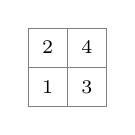
\begin{tikzpicture}[scale=0.5,baseline=12pt] 
	\draw[help lines] (0,0) grid (2,2);
	\node at (.5,.5){$\scriptstyle 1$};
	\node at (.5,1.5){$\scriptstyle 2$};
	\node at (1.5,.5){$\scriptstyle 3$};
	\node at (1.5,1.5){$\scriptstyle 4$};
\end{tikzpicture}
\qquad\text{ and }\qquad
T_2=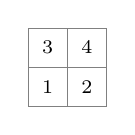
\begin{tikzpicture}[scale=0.5,baseline=12pt] 
	\draw[help lines] (0,0) grid (2,2);
	\node at (.5,.5){$\scriptstyle 1$};
	\node at (.5,1.5){$\scriptstyle 3$};
	\node at (1.5,.5){$\scriptstyle 2$};
	\node at (1.5,1.5){$\scriptstyle 4$};
\end{tikzpicture}\,.
$$
A standard construction of the irreducible of shape  $(2,2)$ from those tableaux $T_1$ and $T_2$
is to apply the Young idempotent associated to $T_i$ to the monomial associated to $T_i$.
That is, $\Delta'_{T_i}=N_{T_i}P_{T_i} \theta_{T_i}=N_{T_i}\theta_{T_i}$
using the action of the symmetric group that we have (namely Hivert action in \cite{H} ).


For $T_1$ and $T_2$ we compute
\begin{align*}
\Delta'_{T_1}&= N_{T_1}\theta_2\theta_4=  \big( Id - (1\, 2)\big)\big( Id - (3\, 4)\big) \theta_2\theta_4 
= \theta_2\theta_4 -  \theta_1\theta_4 -  \theta_2\theta_3 +  \theta_1\theta_3
\\
&=  (\theta_{2}-\theta_{1})(\theta_{4}-\theta_{3}) =\Delta_{C(0101)}
\end{align*}
and
\begin{align*}
\Delta'_{T_2}&= N_{T_2}\theta_3\theta_4=  \big( Id - (1\, 3)\big)\big( Id - (2\, 4)\big) \theta_3\theta_4 
=  \theta_3\theta_4 -  \theta_1\theta_4 -  \theta_2\theta_3 +  \theta_1\theta_2~.
\end{align*}
Remark that for $T_2$, the polynomial $\Delta'_{T_2}$
does not factor into $(\theta_{3}-\theta_{1})(\theta_{4}-\theta_{2})$.
Moreover $\Delta'_{T_2}\notin EQH_n$ and $(\theta_{3}-\theta_{1})(\theta_{4}-\theta_{2})\notin EQH_n$.
 In commutative variable, $\Delta'_{T_2}$ would factor and the  span of the $\{\Delta'_{T_1},\Delta'_{T_2}\}$ (an irreducible module) would  be the same as 
 the span of $\{\Delta_{C(0101)},\Delta_{C(0011)}\}$. But  for anticommutative variables, it is a  different story.
\mike{I think that this whole last paragraph is a good point of discussion for us,
but that it is not a good idea to leave it in the paper.  It seems that it provides
a calculation that doesn't have properties that we would hope to see, but when it doesn't
have those properties it only shows that we didn't make good choices.
Also, there are many actions in
the Hivert paper, which one are you using here (I am guessing the one where we
used the notation $(12) = \pi_1$ and $(34) = \pi_3$, but that wouldn't make it a symmetric
group module.}
\end{remark}



%%%%%%%%%%%%%%%%%%%%%%%%%%%%%%%%%%%%%%
%%%%%%%%%%%%%%%%%%%%%%%%%%%%%%%%%%%%%%
%%%%%%%%%%%%%%%%%%%%%%%%%%%%%%%%%%%%%%
\section{A linear basis of the ring}

Again let $n$ be a fixed positive integer and $R_n = {\mathbb Q}[\theta_1, \theta_2, \ldots, \theta_n]$.
We have thus far represented the basis for
$R_n$ as the elements $\theta_A$ with $A \subseteq [n]$.  Define $\alpha(A) \in \{ 0,1\}^n$ to be
the sequence $a_1 a_2 a_3 \cdots a_n$ with $a_i = 1$ if $i \in A$ and
$a_i = 0$ if $i \notin A$ so that
\[
\theta_A = \theta_1^{a_1} \theta_2^{a_2} \cdots \theta_n^{a_n} := \theta^{\alpha(A)}~.
\]
For such a sequence $\alpha \in \{0,1\}^n$, let $m_1(\alpha) := \sum_{i=1}^n a_i$
represent the number of $1$s in the string.  This will also be the degree of the monomial
$\theta^{\alpha}$.

For sequences $\alpha \in \{ 0, 1 \}^n$, define elements $G_\alpha$ by
\begin{equation}\label{eq:Gdef1}
G_{1^s0^{n-s}} = F_{1^s}
\end{equation}
and if $\alpha \neq 1^s 0^{n-s}$, then $\alpha$ is of the form $u01^s0^{n-k-s}$ for some string $u$
of length $k-1$ and we recursively define
\begin{equation}\label{eq:Gdef2}
G_{u01^s0^{n-k-s}} = G_{u1^s0^{n-k-s+1}} - (-1)^{m_1(u)} \theta_k G_{u1^{s-1}0^{n-k-s+2}}~.
\end{equation}

We will show below that the recurrence for the
$G_\alpha$ are defined so that they are $S$-polynomials \cite{CLO}
for elements of the ideal $I_n$.
In commutative variables, similar polynomials were defined by Aval-Bergeron-Bergeron~\cite{AB,ABB}
as a (complete) subset of $S$-polynomials needed to compute all possible
$S$-polynomials in the Buchburger algorithm for Gr\"obner basis.
It is not given that one can describe easily such a set of $S$-polynomials and here we have adapted
the definition for working in the exterior algebra.

\begin{example} For $\alpha = 010110$ and $\beta = 001100$, we compute
the elements $G_\alpha$ and $G_\beta$ using the definition.
\begin{align*}
G_{010110} &= G_{011100} + \theta_3 G_{011000} = (G_{111000} - \theta_1 G_{110000})
+ \theta_3(G_{110000} - \theta_1 G_{100000})\\
&= \theta_2 \theta_4 \theta_5 + \theta_2 \theta_4 \theta_6 + \theta_2 \theta_5 \theta_6
+ 2 \theta_3 \theta_4 \theta_5 + 2 \theta_3 \theta_4 \theta_6 + 2 \theta_3 \theta_5 \theta_6
+ \theta_4 \theta_5 \theta_6
\end{align*}

and we have that
\begin{align*}
G_{001100} &= G_{011000} - \theta_2 G_{010000} = (G_{110000} - \theta_1 G_{100000})
- \theta_2 (G_{100000} - \theta_1 G_{000000})\\
&= \theta_3 \theta_4 + \theta_3 \theta_5 + \theta_3 \theta_6 + \theta_4 \theta_5 + \theta_4 \theta_6 + \theta_5 \theta_6
\end{align*}
\end{example}

Order the monomials of $R_n$ so that we say $\theta_A < \theta_B$ if
$\alpha(A)$ is smaller than $\alpha(B)$ in lexicographic order.
An important property of these elements is the following statement.
\mike{todo: define clearly the order and wherever we use the term `lexicographic',
make sure it is used properly}
\begin{prop}\label{prop:largest}
The largest lexicographic term in $G_\alpha$ is $\theta^\alpha$.
\end{prop}

The proof of Proposition \ref{prop:largest} follows by induction
on the length of $\alpha$ and
from a lemma that is analogous to Lemma 3.3 of \cite{AB}.
The recursion in this result is really the origin of the definition
of $G_\alpha$ because Equation \eqref{eq:Gdef2}
was adapted so that this lemma holds.  It follows that
the set $\{ G_\alpha \}_{\alpha \in \{0,1\}^n}$ is a basis
for $R_n$.

The argument for the proposition is elementary (chasing the largest lexicographic
term in \eqref{eq:0start} and \eqref{eq:1start})
and so we do not include it, however the proof of the
following result comes from careful analysis of the
terms arising the recursive definition of the $G_\alpha$.

\begin{lemma}\label{lem:LT}
 Let $\alpha \in \{0,1\}^{n-1}$, then
\begin{align}
G_{0\alpha} &= G_\alpha(\theta_2, \theta_3, \ldots, \theta_n) \hbox{ and }\label{eq:0start}\\
G_{1\alpha} &= \theta_1 G_{0\alpha} + P_{\alpha}(\theta_2, \theta_3, \ldots, \theta_n)\,. \label{eq:1start}
\end{align}
\end{lemma}

\begin{remark}\label{rem:shift}
By convention, the length of the index for our polynomials indicate in which polynomial space we are.
For example if $\beta   \in \{0,1\}^{n}$ then $G_\beta\in R_n$. For $\alpha \in \{0,1\}^{n-1}$  in Lemma~\ref{lem:LT}, when we write
$G_\alpha(\theta_2, \theta_3, \ldots, \theta_n)$ we mean $G_\alpha\in  R_{n-1}$
embedded in $R_n$ with the substitution
$\theta_i:=\theta_{i+1}$. A similar convention will be followed for $P_\alpha$.
\end{remark}

\begin{proof}[Proof of Lemma~\ref{lem:LT}]
The proof will be by induction on $n-i$ where $i$ is the number of trailing $0$s in $\alpha$.
The base case $0=n-n$ with $n$ zeros, is $0\alpha = 0^n$ and we have
\[
G_{0^n} = F_{1^0}(\theta_1,\theta_2 ,\ldots,\theta_n) = 1
= G_{0^{n-1}}(\theta_2, \theta_3, \ldots, \theta_n)~.
\]
We then consider the case  $0\alpha=01^s0^{n-s-1}$. The polynomials $F_{1^s}$ satisfy the  following identity
\begin{equation}\label{eq:relF}
F_{1^s}(\theta_1,\theta_2 ,\ldots,\theta_n)
= \theta_1 F_{1^{s-1}}(\theta_2 ,\ldots,\theta_n) + F_{1^s}(\theta_2,\theta_3 ,\ldots,\theta_n)
\end{equation}
This follows directly from the definition~\eqref{eq:defF} where we split the sum in two parts depending if $1\in A$ or not.
The definition of $G_{01^s0^{n-s-1}}$  gives us
\begin{align*}
	G_{01^s0^{n-s-1}}&= G_{1^s0^{n-s}} - \theta_1 G_{1^{s-1}0^{n-s+1}}
	  =F_{1^s}(\theta_1,\theta_2 ,\ldots,\theta_n) - \theta_1 F_{1^{s-1}}(\theta_2 ,\ldots,\theta_n) \\
	  &= F_{1^s}(\theta_2,\theta_3 ,\ldots,\theta_n)= G_{\alpha}(\theta_2,\theta_3 ,\ldots,\theta_n)\,.
\end{align*}

To finish the  proof of Equation~\eqref{eq:0start} by induction,
let us assume that $\alpha$ is not of the form
$01^s0^{n-s-1}$ for some $s>0$.
Instead we have $0\alpha=0w01^s0^{n-k-s}$ for some $s>0$ and some string $w$
of length $k-2$.
For $0\alpha=0w01^s0^{n-k-s}$, we have $n-k-s$ trailing zeros.
Remark that for $0w1^s0^{n-k-s+1}$ and $0w1^{s-1}0^{n-k-s+2}$
we have more trailing zeros than appear in $0\alpha$ and we will use the
induction hypothesis (with~\eqref{eq:0start}) in the
equality~\eqref{eq:IH0} below.%%%%%%%
\begin{align}
	G&_{0w01^s0^{n-k-s}}= G_{0w1^s0^{n-k-s+1}} -  (-1)^{m_1(0w)} \theta_k G_{0w1^{s-1}0^{n-k-s+2}} \nonumber \\
	 & = G_{w1^s0^{n-k-s+1}}(\theta_2,\theta_3 ,\ldots,\theta_n) - (-1)^{m_1(0w)} \theta_k G_{w1^{s-1}0^{n-k-s+2}}(\theta_2,\theta_3 ,\ldots,\theta_n) \label{eq:IH0}\\
	 & = \big[G_{w1^s0^{n-k-s+1}} - (-1)^{m_1(w)} \theta_{k-1} G_{w1^{s-1}0^{n-k-s+2}}\big](\theta_2,\theta_3 ,\ldots,\theta_n)\label{eq:detail0}\\
	 & = G_{w01^s0^{n-k-s}} (\theta_2,\theta_3 ,\ldots,\theta_n)
	   = G_{\alpha} (\theta_2,\theta_3 ,\ldots,\theta_n)  \label{eq:final0}
\end{align}
In~\eqref{eq:detail0} the expression inside the square bracket $[\cdots]$ is as polynomials in the variables $\theta_1,\ldots,\theta_{n-1}$ in $R_{n-1}$ (see Remark~\ref{rem:shift}).
Hence, the variable $\theta_{k}$ from \eqref{eq:IH0} must
be replaced by $\theta_{k-1}$ in \eqref{eq:detail0}.
Also, $m_1(0w)=m_1(w)$. The expression we get is exactly the definition of
$G_{w01^s0^{n-k-s}} \in R_{n-1}$ and Equation~\eqref{eq:final0} follows.
This concludes the proof of \eqref{eq:0start}.

We next prove Equation \eqref{eq:1start} by induction.  The base case is if $1\alpha = 1^{s+1}0^{n-s-1}$,
then using Equation \eqref{eq:relF} we have
\begin{align}
G_{1^{s+1}0^{n-s-1}} &= F_{1^{s+1}}(\theta_1,\theta_2 ,\ldots,\theta_n) \nonumber\\
&= \theta_1 F_{1^s} (\theta_2, \theta_3, \ldots, \theta_n)+ F_{1^{s+1}}(\theta_2, \theta_3, \ldots, \theta_n)\nonumber \\
&= \theta_1 G_{01^s0^{n-s-1}} + F_{1^{s+1}}(\theta_2, \theta_3, \ldots, \theta_n)~.\label{eq:base1}
\end{align}
In~\eqref{eq:base1}, we use \eqref{eq:0start} with  $G_{01^s0^{n-s-1}}=G_{1^s0^{n-s-1}} (\theta_2,  \ldots, \theta_n)=F_{1^s} (\theta_2, \ldots, \theta_n)$.
We then let
$P_{1^{s}0^{n-s-1}} = F_{1^{s+1}}(\theta_1,\ldots,\theta_{n-1})$ and this shows that \eqref{eq:1start} holds in this case.

We now assume that $1\alpha\ne 1^{s+1}0^{n-s-1}$. Therefore $1\alpha=1w01^s0^{n-k-s}$ for some string $w$
of length $k-2$. We have
\begin{align}
	G&_{1w01^s0^{n-k-s}}= G_{1w1^s0^{n-k-s+1}} -  (-1)^{m_1(1w)} \theta_k G_{1w1^{s-1}0^{n-k-s+2}} \nonumber \\
	 & = \big(\theta_1G_{0w1^s0^{n-k-s+1}} +P_{w1^s0^{n-k-s+1}}(\theta_2,\theta_3 ,\ldots,\theta_n)\big) \label{eq:IH1}\\
	 &\qquad\qquad  - (-1)^{m_1(1w)} \theta_k  \big(\theta_1G_{0w1^{s-1}0^{n-k-s+2}} +P_{w1^{s-1}0^{n-k-s+2}}(\theta_2,\theta_3 ,\ldots,\theta_n)\big) \nonumber\\
	 & = \theta_1\big(G_{0w1^s0^{n-k-s+1}}   - (-1)^{m_1(w)}  \theta_k G_{0w1^{s-1}0^{n-k-s+2}}\big)	 \label{eq:detail1}\\
	 &\qquad\qquad  + \big[P_{w1^s0^{n-k-s+1}}  - (-1)^{m_1(1w)} \theta_{k-1} P_{w1^{s-1}0^{n-k-s+2}}\big] (\theta_2,\theta_3 ,\ldots,\theta_n)\nonumber
%	 & = \theta_1 G_{0\alpha} + P_\alpha(\theta_2, ,\theta_3 ,\ldots,\theta_n)  \nonumber
\end{align}
In \eqref{eq:IH1}, we have used the induction hypothesis of~\eqref{eq:1start} on both terms.
In  \eqref{eq:detail1}, we group together the terms with $\theta_1$ in front, using the identity
$(-1)^{m_1(1w)} \theta_k \theta_1 = (-1)^{m_1(1w)+1} \theta_1 \theta_k  = (-1)^{m_1(w)} \theta_1 \theta_k $.
The term with $\theta_1$ in \eqref{eq:detail1} is the definition of $G_{0\alpha}$.
The expression inside the square bracket is a polynomial in $R_{n-1}$ that we take as the definition for $P_\alpha$.
This shows by induction that \eqref{eq:1start}
holds in all cases and concludes the  proof of the lemma.
\end{proof}


%%%%%%%%%%%%%%%%%%%%%%%%%%%%%%%%%%%%%%
%%%%%%%%%%%%%%%%%%%%%%%%%%%%%%%%%%%%%%
%%%%%%%%%%%%%%%%%%%%%%%%%%%%%%%%%%%%%%
\section{A path model for the quotient}\label{sec:path}

To each sequence $\alpha \in \{0, 1\}^n$, we associate a path starting at the origin
and extending into the first quadrant of the $x,y$-plane.  The $i^{th}$ step of this
path will be a unit in the $(1,0)$-direction if $a_i =1$ and it will be a unit in the $(0,1)$-direction
if $a_i = 0$.  We say that the sequence $\alpha$ \defn{crosses the diagonal} if
there is a point on the path which lies at $(a,a)$ and the next step is in the $(1,0)$
direction.  Otherwise we say that $\alpha$ \defn{stays above the diagonal}.  Note that
$\alpha$ stays above the diagonal if $\sum_{i=1}^r a_i \leq r/2$
for all $1 \leq r \leq n$
and it crosses the diagonal otherwise. The ballot sequences we encountered earlier are the one that  stay above the diagonal.

\begin{example} Let $n=6$ and $\alpha = 010110$ and $\beta = 001100$, then the corresponding
paths are
\begin{center}
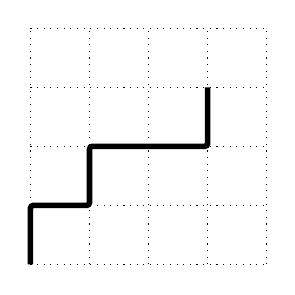
\begin{tikzpicture}[scale=.75]
  \draw[dotted] (0, 0) grid (4, 4);
  \draw[rounded corners=1, color=black, line width=2] (0, 0) -- (0, 1) -- (1, 1) -- (1, 2) -- (2, 2) -- (3, 2) -- (3, 3);
\end{tikzpicture}
\hskip .5in
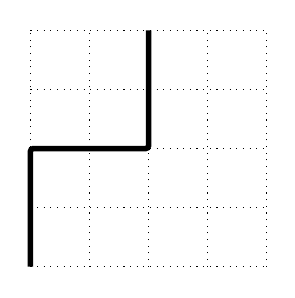
\begin{tikzpicture}[scale=.75]
  \draw[dotted] (0, 0) grid (4, 4);
  \draw[rounded corners=1, color=black, line width=2] (0, 0) -- (0, 1) -- (0, 2) -- (1, 2) -- (2, 2) -- (2, 3) -- (2, 4);
\end{tikzpicture}
\end{center}
\end{example}

The elements $G_\alpha$ are defined so that we could use them to
identify a nice basis of the ideal $I_n$.  Our first result establishes
that the $G_\alpha$ such that $\alpha$ crosses the diagonal
are in the ideal.  The slightly more difficult step is to show
that these elements also span the ideal.

\begin{prop}\label{prop:crossimpliescontains}
If $\alpha$ crosses the diagonal, then $G_\alpha \in I_n$.
\end{prop}

\begin{proof}
A sequence $\alpha \in \{ 0, 1\}^n$ is either of the form
$\alpha = 1^s0^{n-s}$ for some $s > 0$ or
$\alpha = u01^s0^{n-s-k}$ for some $s>0$ and some $u \in \{0,1\}^{k-1}$.

In the first case, $\alpha$ crosses the diagonal on the first step and
by Equation \eqref{eq:Gdef1}, $G_{1^s0^{n-s}} = F_{1^s}$
is in the ideal $I_n$.

Now the other case is established by
induction on the position of the last $1$ in $\alpha$.
We assume that
$\alpha = u01^s0^{n-s-k}$ and, by Equation \eqref{eq:Gdef2},
$G_\alpha$ is in $I_n$ if both
$G_{u1^s0^{n-k-s+1}}$ and $G_{u1^{s-1}0^{n-k-s+2}}$
are elements of $I_n$.

Assume that $u01^s0^{n-s-k}$
crosses the diagonal for the first time at position $r$.
If $r<k$, then
$u1^s0^{n-k-s+1}$ and $u1^{s-1}0^{n-k-s+2}$
both cross the diagonal also at position $r$.
Since $\alpha_k=0$, $\alpha$ does not cross the diagonal for the first
time at $r=k$, so the other possibility is that is $r>k$.
In this case $u01^{r-k}$ with $r-k \leq s$ crosses the diagonal for the first time
and therefore so does $u1^{r-k-1}$ and so do both
$u1^s0^{n-k-s+1}$ and $u1^{s-1}0^{n-k-s+2}$.
By our inductive hypothesis this implies $G_\alpha \in I_n$.

Therefore by induction, $\alpha$ crosses the diagonal implies $G_\alpha \in I_n$
for all $\alpha \in \{0,1\}^n$.
\end{proof}

We will  show that the ideal lies in the span of the $G_\alpha$ such
that $\alpha$ crosses the diagonal therefore establishing our main theorem.

\begin{theorem}\label{thm:basisofideal}
The set $A_n:=\big\{ G_\alpha : \alpha \in \{0,1\}^n \text{ \it crosses the diagonal}\big\}$
is a $\mathbb Q$--linear basis of the ideal $I_n$.
\end{theorem}

The proof of this theorem uses our understanding of the harmonic space $EQH_n\cong EQC_n$.
In Proposition~\ref{prop:harmbasis} we found that $\dim(EQH_n)=\dim(EQC_n)$ is at least the number of ballot sequences.
We first establish a small lemma about a spanning set for the quotient $EQC_n$ showing that  the dimension is at most  the number of ballot sequences.
Therefore we have equality
and the set ${\mathcal D}_n$ in Proposition~\ref{prop:harmbasis} is in fact a basis
of $EQH_n$.


\begin{lemma}\label{lem:spanofquotient}
The set $B_n=\big\{ \theta^\beta : \beta \in \{0,1\}^n \text{ \it stays above the diagonal}\big\}$
$\mathbb Q$--spans the quotient $R_n\big/I_n$.
\end{lemma}

\begin{proof}
Order the monomials lexicographically. Let  $\theta^\gamma$ be the smallest monomial that is not in the $\mathbb Q$--span of $B_n$
(modulo  $I_n$). We must have  that $\gamma$ crosses the  diagonal, since otherwise $\theta^\gamma\in  B_n$. Therefore, Proposition~\ref{prop:crossimpliescontains}
tells us  that $G_\gamma \in I_n$. Proposition~\ref{prop:largest} say that $G_\gamma = \theta^\gamma + \sum_{\beta<\gamma}  c_\beta \theta^\beta$. Hence, modulo $I_n$, we have
$$ \theta^\gamma \equiv \theta^\gamma - G_\gamma = - \sum_{\beta<\gamma} c_\beta \theta^\beta\,.$$
The right hand side is a linear combination of monomials strictly smaller than $\theta^\gamma$.
By the choice of $\theta^\gamma$, all such monomials are in the $\mathbb Q$--span of $B_n$.
 Therefore $\theta^\gamma$ is also in the $\mathbb Q$--span of $B_n$, a contradiction. We must conclude there are no such $\theta^\gamma$ and all monomials are in the $\mathbb Q$--span of $B_n$ modulo the ideal $I_n$.
\end{proof}

\begin{proof}[Proof of Theorem~\ref{thm:basisofideal}]
Let $d_n$ be the number of ballot sequences of size $n$. We also have that this is exactly the set of sequence $\alpha\in\{0,1\}^n$ that stays above the  diagonal.
We have
$$ d_n\le \dim EQH_n = \dim EQC_n \le d_n,$$
where the first inequality is using Proposition~\ref{prop:harmbasis} and second follow from Lemma~\ref{lem:spanofquotient}.
Let ${\mathbb Q}A_n$ be the ${\mathbb Q}\text{-span}$ of the elements of $A_n$.
Similarly, let ${\mathbb Q}B'_n$ be the ${\mathbb Q}\text{-span}$ of the set $\big\{ G_\beta : \beta \in \{0,1\}^n \text{ \it stays above the diagonal}\big\}$.
Using Proposition~\ref{prop:largest} we have that
$$R_n ={\mathbb Q}B'_n \oplus  {\mathbb Q}A_n 
$$
Since ${\mathbb Q}A_n \subseteq I_n$ and $\dim {\mathbb Q}B'_n = d_n$, we conclude that ${\mathbb Q}A_n = I_n\,.$
\end{proof}

There are several straightforward consequence of this theorem which we state here.

\begin{cor} The set ${\mathcal D}_n$ is a basis of $EQH_n$ and of $EQC_n$.
\end{cor}

\begin{cor} The set $A_n$ is a (non-reduce, non minimal) Gr\"obner basis of $I_n$. A minimal Gr\"obner basis for $I_n$ is given by
$$ I_n =\big\{ G_\alpha : \alpha \in \{0,1\}^n \text{ \it crosses the diagonal only  at the rightmost  1 of }  \alpha\big\}\,.
$$
\end{cor}


\vskip 1in

\begin{thebibliography}{999}

\bibitem{AB} J. C. Aval, N. Bergeron,
\textit{Catalan paths and quasi-symmetric functions}.
Proc. of the Am. Math. Soc., 2003, 131(4), pp. 1053--1062.
\href{https://doi.org/10.1090/S0002-9939-02-06634-0}{10.1090/S0002-9939-02-06634-0}.

\bibitem{ABB} J. C. Aval, F. Bergeron, N. Bergeron,
\textit{Ideals of quasi-symmetric functions and super-covariant polynomials for $S_n$}.
Adv. in Math., 2004, 181 (2), pp. 353--367.
\href{https://doi.org/10.1016/S0001-8708(03)00068-9}{10.1016/S0001-8708(03)00068-9}.

\bibitem{CLO} D. Cox, J. Little, D. O'Shea,
\textit{Ideals, varieties, and algorithms: an introduction to computational
algebraic geometry and commutative algebra}.
Springer Science \& Business Media; 2013 Mar 9.

\bibitem{FLP}
Susanna Fishel, Luc Lapointe and Mar\'{\i}a Elena Pinto,
\textit{Hopf algebra structure of symmetric and quasisymmetric
              functions in superspace}.
 {J. Combin. Theory Ser. A}, 2019, 166, pp.  {144--170}.
\href{https://doi-org/10.1016/j.jcta.2019.02.016}{10.1016/j.jcta.2019.02.016}.

\bibitem{H} F. Hivert,
\textit{Hecke algebras, difference operators, and quasi-symmetric
              functions}.
Adv. in Math., 2000, 155 (2), pp. 181--238.
\href{https://doi-org/10.1006/aima.1999.1901}{10.1006/aima.1999.1901}.

\bibitem{L} S. X. Li,
\textit{Ideals and quotients of diagonally quasi-symmetric functions}.
Elec. J. Comb., Vol 24, Issue \#3, P3.3.
\href{https://doi.org/10.37236/6658}{10.37236/6658}.

\bibitem{OEIS} OEIS Foundation Inc. (2022),
The On-Line Encyclopedia of Integer Sequences, Published electronically at
\href{http://oeis.org}{http://oeis.org}.
\end{thebibliography}

\end{document}
